\chapter{Theory}
This chapter will presents theoretic concepts that help understand the methodologies used during the course of this project. First, the reader will be presented with fundamental concepts related autonomous mobile robotics. Then, theory about robotic manipulation and tag based machine vision will be explained. Finally, ROS2 is explained, as this is a vital part of the project.
% aj - presents. Not is future but in simple present tense. something like this
% This chapter presents the ovelying thoery behind the autonomous warehous functionalities namely ... a,b,c .. in chapter 1. Starting with the fundamental conpept of use of unmanned ground vehicle (UGV) for warehouse automation, then we describe the autonomous navigation ......Finally we intergrate individual functionalities to achieve warehouse automation.

\section{Autonomous Navigation}
As pointed out in section \ref{sec:I:AutonomousNavigation}, for a mobile robot to be able to do autonomous navigation, four building blocks has to be fulfilled, or rather, four problems has to be solved. This section describes methods used to solve these problems in mobile robotics.

\subsection{Motion Control}
Motion Control refers to the actuation of motors to move around the environment in a controlled manner. The control system calculates the actuation of the robotic motors based on forward kinematics, moves the mobile robot by actuating its motors and calculates its movement based on wheel measurements and inverse kinematics.

Close to all mechanisms of locomotion are heavily inspired from nature. Examples of such locomotion mechanisms are walking, sliding, jumping, swimming and flying. However, there is one type of locomotion invented by humans that is also extremely energy efficient on hard surfaces; the powered wheel. Legged locomotion gives the benefit of adaptability and manoeuvrability in rough terrain. However, legged locomotion suffer from power inefficiency and high complexity. Wheeled locomotion is therefore by far the most popular type of locomotion in mobile robotics\cite{SiegwartRoland2011Itam}.

\subsubsection{Differential Drive Robots}
Differential drive mobile robots refers to a wheeled robotic system made up of a rigid body with two driven wheels. Figure \ref{fig:differentialDrive} illustrates different types of differential drive robotic movement systems. The common denominator for all three of the robotic systems in figure \ref{fig:differentialDrive}, is that they all rely on two driven wheels.

\begin{figure}[H]
  \centering
  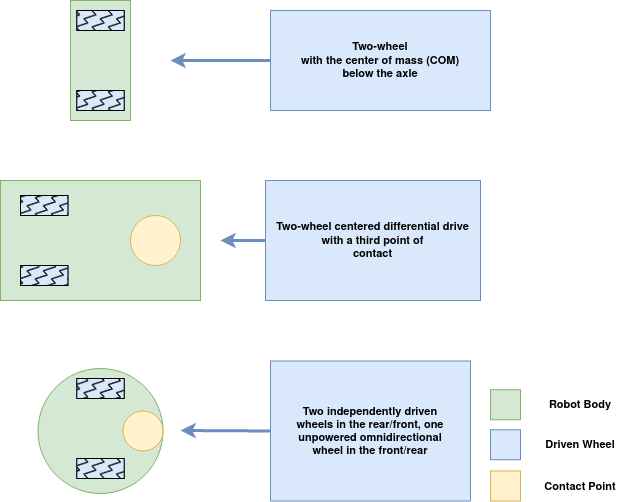
\includegraphics[width = 0.7\textwidth]{Figures/DifferentialDrive.drawio.png}
  \caption{Illustration of different differential drive robotic designs. \textbf{1:} Two independently driven wheels in the rear/front, one unpowered omnidirectional wheel in the front/rear. \textbf{2:} Two-wheel centered differential drive with a third point of contact. \textbf{3:} Two-wheel differential drive with the center of mass (COM) below the axle. Figure inspired from \cite{SiegwartRoland2011Itam}.}
  \label{fig:differentialDrive}
\end{figure}

The robot is modeled as a rigid body on wheels, interacting with a horizontal plane. The robot has a total of three DOFs, two for postion, and one orientaion along the orthogonal axis of the plane. Figure FIGURE! illustrates how the robot is modeled and its  positional notation relative to the reference frame.





\subsection{Perception}
Talk about lidar systems
\subsubsection{LiDAR}
Light Detection and Ranging sensors, are sensors that utilise light and time-of-flight principle to determine the distance from a sensor to an obstacle. 

\subsubsection{Camera or Radar maybe?}


\subsection{Localisation \& Mapping}


\subsubsection{Inertial Measurement Unit}


\subsubsection{Adaptive Monte Carlo Localisation}


\subsubsection{Simultaneous Localisation And Mapping}
This section describes different localisation and mapping methodologies, specifically Simultaneous Localisation And Mapping(SLAM) and Adaptive Monte Carlo Localisation(AMCL). SLAM is a localisation and mapping method that simultaneously generates a map of it's environment as it does the localisation. AMCL is a particle-based localisation algorithm that is often used in robotics to determine the location of a robot in it's environment.

\section{Robotic Manipulation}
Moveit 2 is an open-source robot manipulator planning and manipulation framework based on ROS 2. It provides tools like anti-collision and gives robotic manipulators using  ROS 2 a robust platform for manipulation. Integration with ROS 2 means that this framework is widely used within the robotics community

\section{Tag Based 3D Machine Vision}\label{sec:T:TagBased3DMachineVision}
AprilTags are a system of visual tags developed by researchers at the University of Michigan to provide low overhead, high accuracy localisation for many different applications. 

\section{Robot Operating System 2}
Robot operating system 2 is an open source operating system for robots that is aimed at simplifying the communication between different sensors and actuators in a robotic system, and present the information from these different sensors and actuators in a standardised matter.

\subsection{URDF}


\subsection{Navigation 2}
Navigation 2(NAV 2) is a open-source navigation stack based on ROS 2. It's modular design is made to provide a robust navigation platform for robots utilising ROS 2.
